\section{Fordeling af besvarelserne}
\label{TestAfSkalaFordelingAfBesvarelserne}
%
Fra dette afsnit laves en henvisning til dokumentet med oversigten over fordelingen af besvarelser for besvarelserne til hver af skalaerne. (Som kommer til at ligge i elektronisk bilag)
%
\begin{figure}[H]
\centering
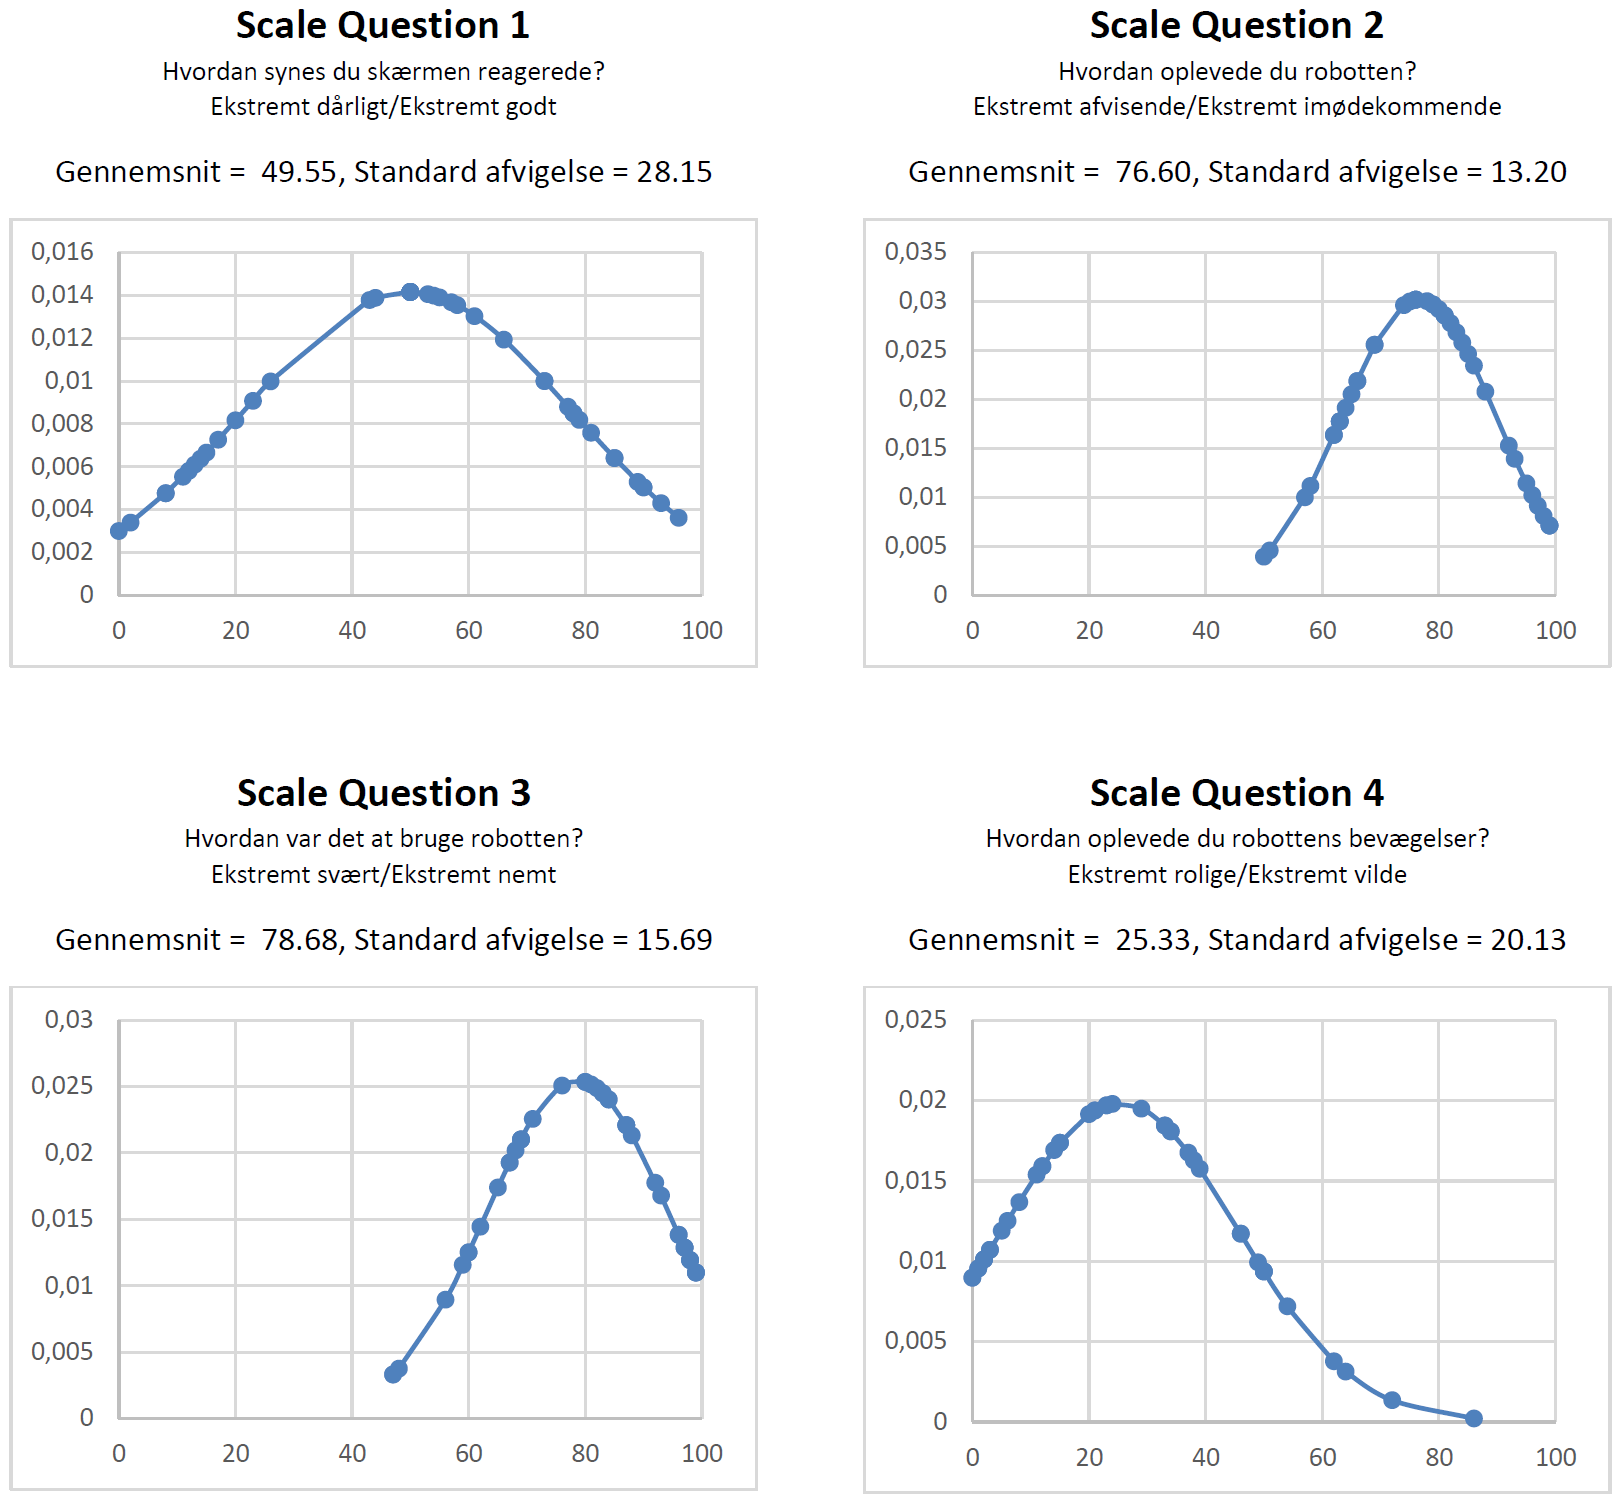
\includegraphics[width =\textwidth]{Figure/DatabehandlingSkalaer/FordelingSkala1_4} 
\caption{Fordelingen af besvarelserne til Scale Question 1-4}
\label{fig:FordelingSkala1_4}
\end{figure}
\noindent
%
Kigger man på scale question 1 (SQ1) i \autoref{fig:FordelingSkala1_4} fremgår det ret tydeligt, at skærmen ikke har reageret godt for alle, hvilket stemmer overens med vores observationer. Data fordeler sig groft i tre grupper: 0-30, 40-70 og 70-100. Det er til gengæld en af de mest klokkeformede fordelinger i forhold til de andre i datasættet. Kigges på SQ2 og SQ3 virker det ikke til, at hele skalaen har været i brug og besvarelserne klumper sammen fra midterpunktet og op. Det kan tilgengæld ses som værende positivt, da folk generelt har ment, at robotten har været meget imødekommende og nem at bruge. På SQ4 virker data til at være lettere skævvreden til højre. Det betyder, at de fleste har oplevet robottens bevægelser som rolige, men der er lidt uenighed, da der også er en del besvarelser, der ligger i den vilde ende.

\begin{figure}[H]
\centering
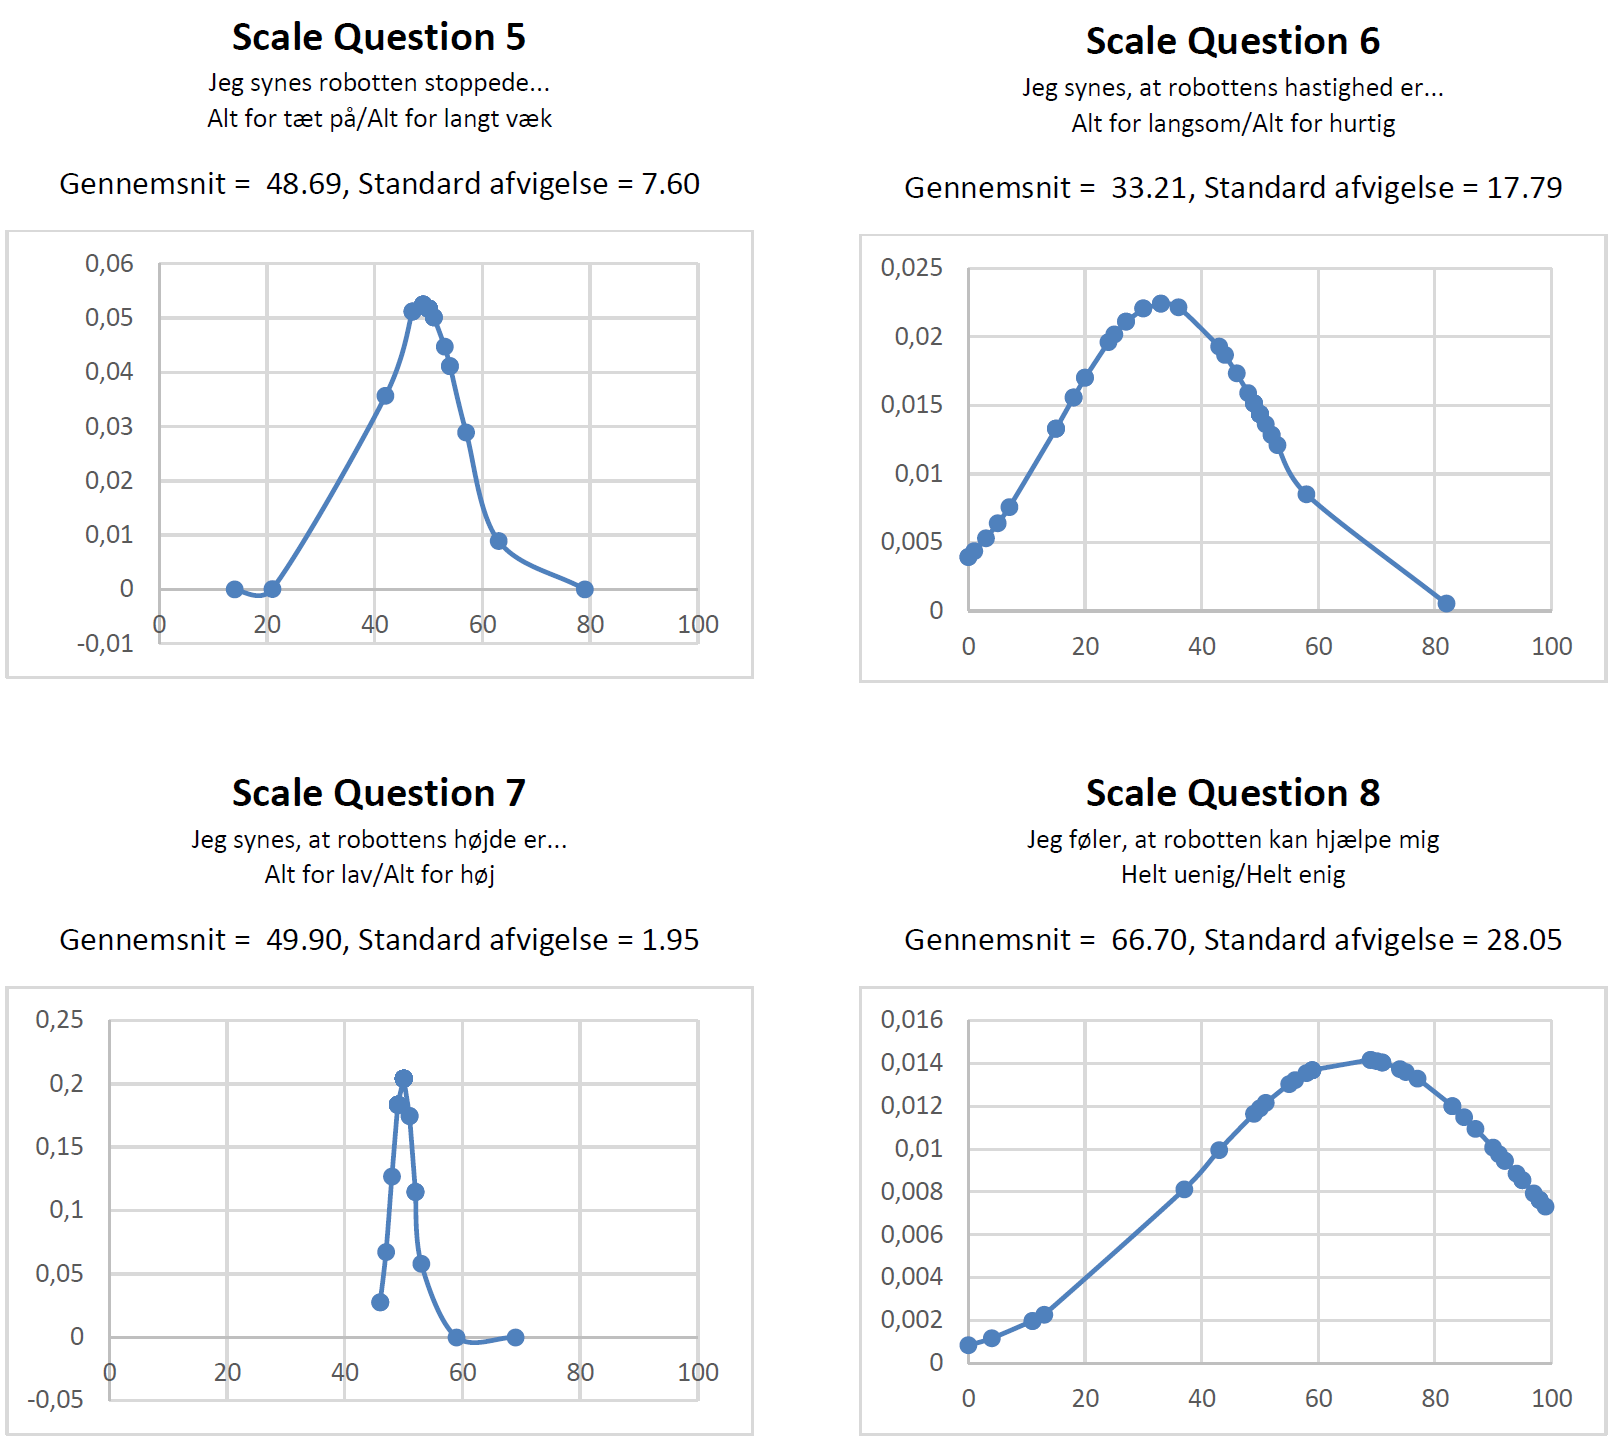
\includegraphics[width =\textwidth]{Figure/DatabehandlingSkalaer/FordelingSkala5_8} 
\caption{Fordelingen af besvarelserne til Scale Question 5-8}
\label{fig:FordelingSkala5_8}
\end{figure}
\noindent

På \autoref{fig:FordelingSkala5_8} handlede SQ5 om, hvor tæt robotten stoppede på personen. Det blev observeret undervejs at folk let misforstod spørgsmålet således, at det drejede sig om, hvor tæt robotten stoppede på deres valgte destination, hvilket de selvfølgelig ikke kunne svare på. Det fremgår måske også af, at mange besvarelse ligger lige omkring midten og standardafvigelsen er lille (SD=7.6). Meget få synes, at robottens hastighed er for hurtig, hvilket fremgår af SQ6.  Hastigheden på robotten varierede i takt med højden, da robotten kører langsommere, når højden hæves. Det virker til, at den sagtens kunne blive en smule hurtigere. Den absolut mindste standardafvigelse ses til SQ7, der spørger ind til højden (SD=1.95). Her er langt de fleste besvarelser sat i midten, hvilket resulterer i en meget spids fordeling. Det kan betyde, at folk ikke tænker så meget over højden eller det kan betyde, at labelen "fin" på midterpunktet har været alt for bredt dækkende og derfor ikke er et passende midtpunkt.\\
SQ8 virker skævvreden til venstre, hvilket kunne tyde på, at skalaen ikke har været bred nok, da højre ende punkt ikke virker ekstremt nok.

\begin{figure}[H]
\centering
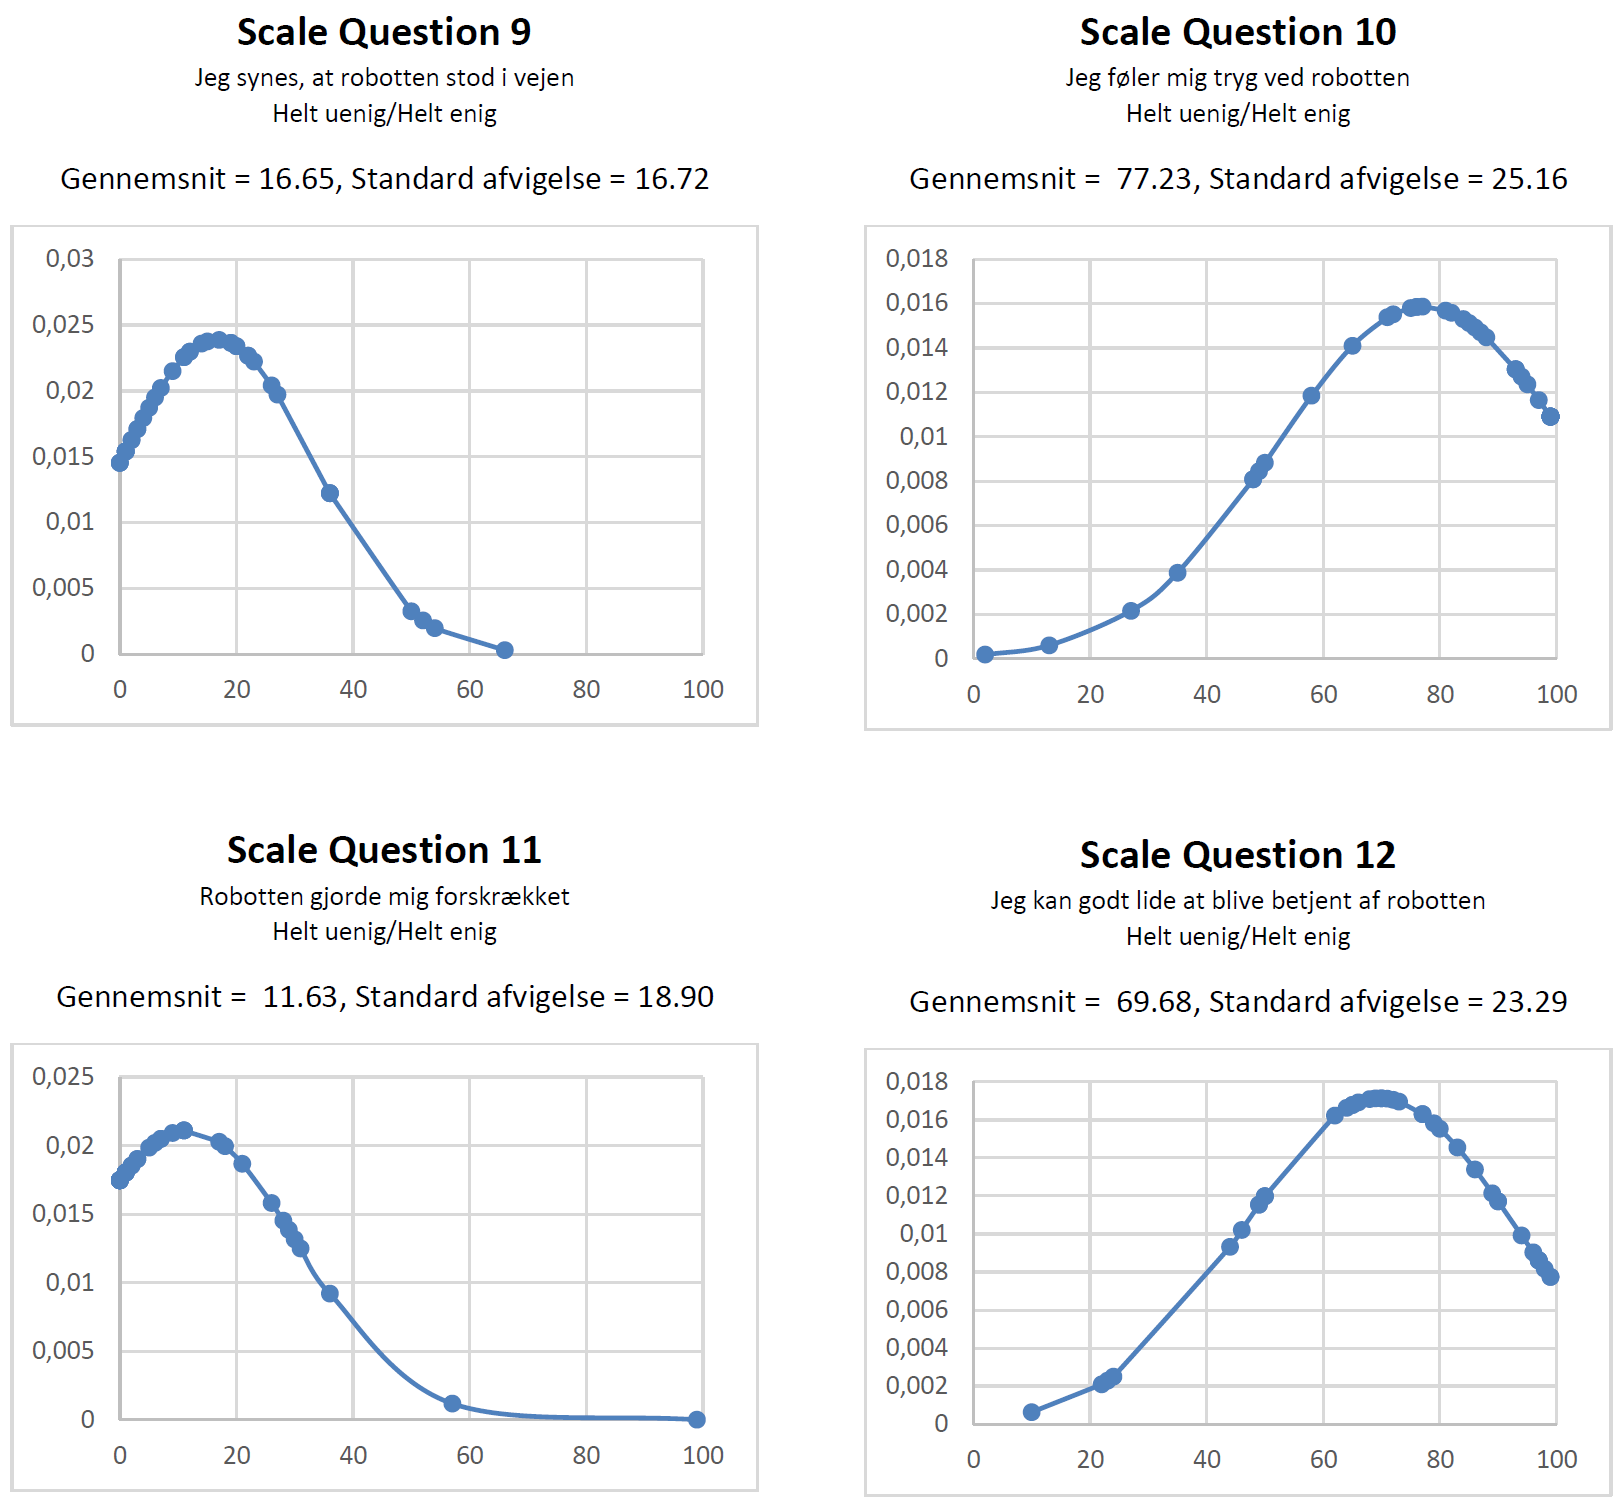
\includegraphics[width =\textwidth]{Figure/DatabehandlingSkalaer/FordelingSkala9_12} 
\caption{Fordelingen af besvarelserne til Scale Question 9-12}
\label{fig:FordelingSkala9_12}
\end{figure}
\noindent

På \autoref{fig:FordelingSkala9_12} ses samme tendens som SQ4 og SQ8, da fordelingerne er skævvredne. SQ9 og SQ11 er højre skævvreden hvor SQ10 og SQ12 er venstre skævvreden.  Det kan muligvis skyldes endepunkterne på skalaerne, hvilket i dette tilfælde er "Helt enig/Helt uenig". Generelt virker robotten ikke til at have stået i vejen eller at gøre folk forskrækket. Folk kan generelt godt lide at blive betjent af robotten og føler sig trygge ved den. Der er dog få, der er uenige, hvilket skaber lidt skæve fordelinger.


\begin{figure}[H]
\centering
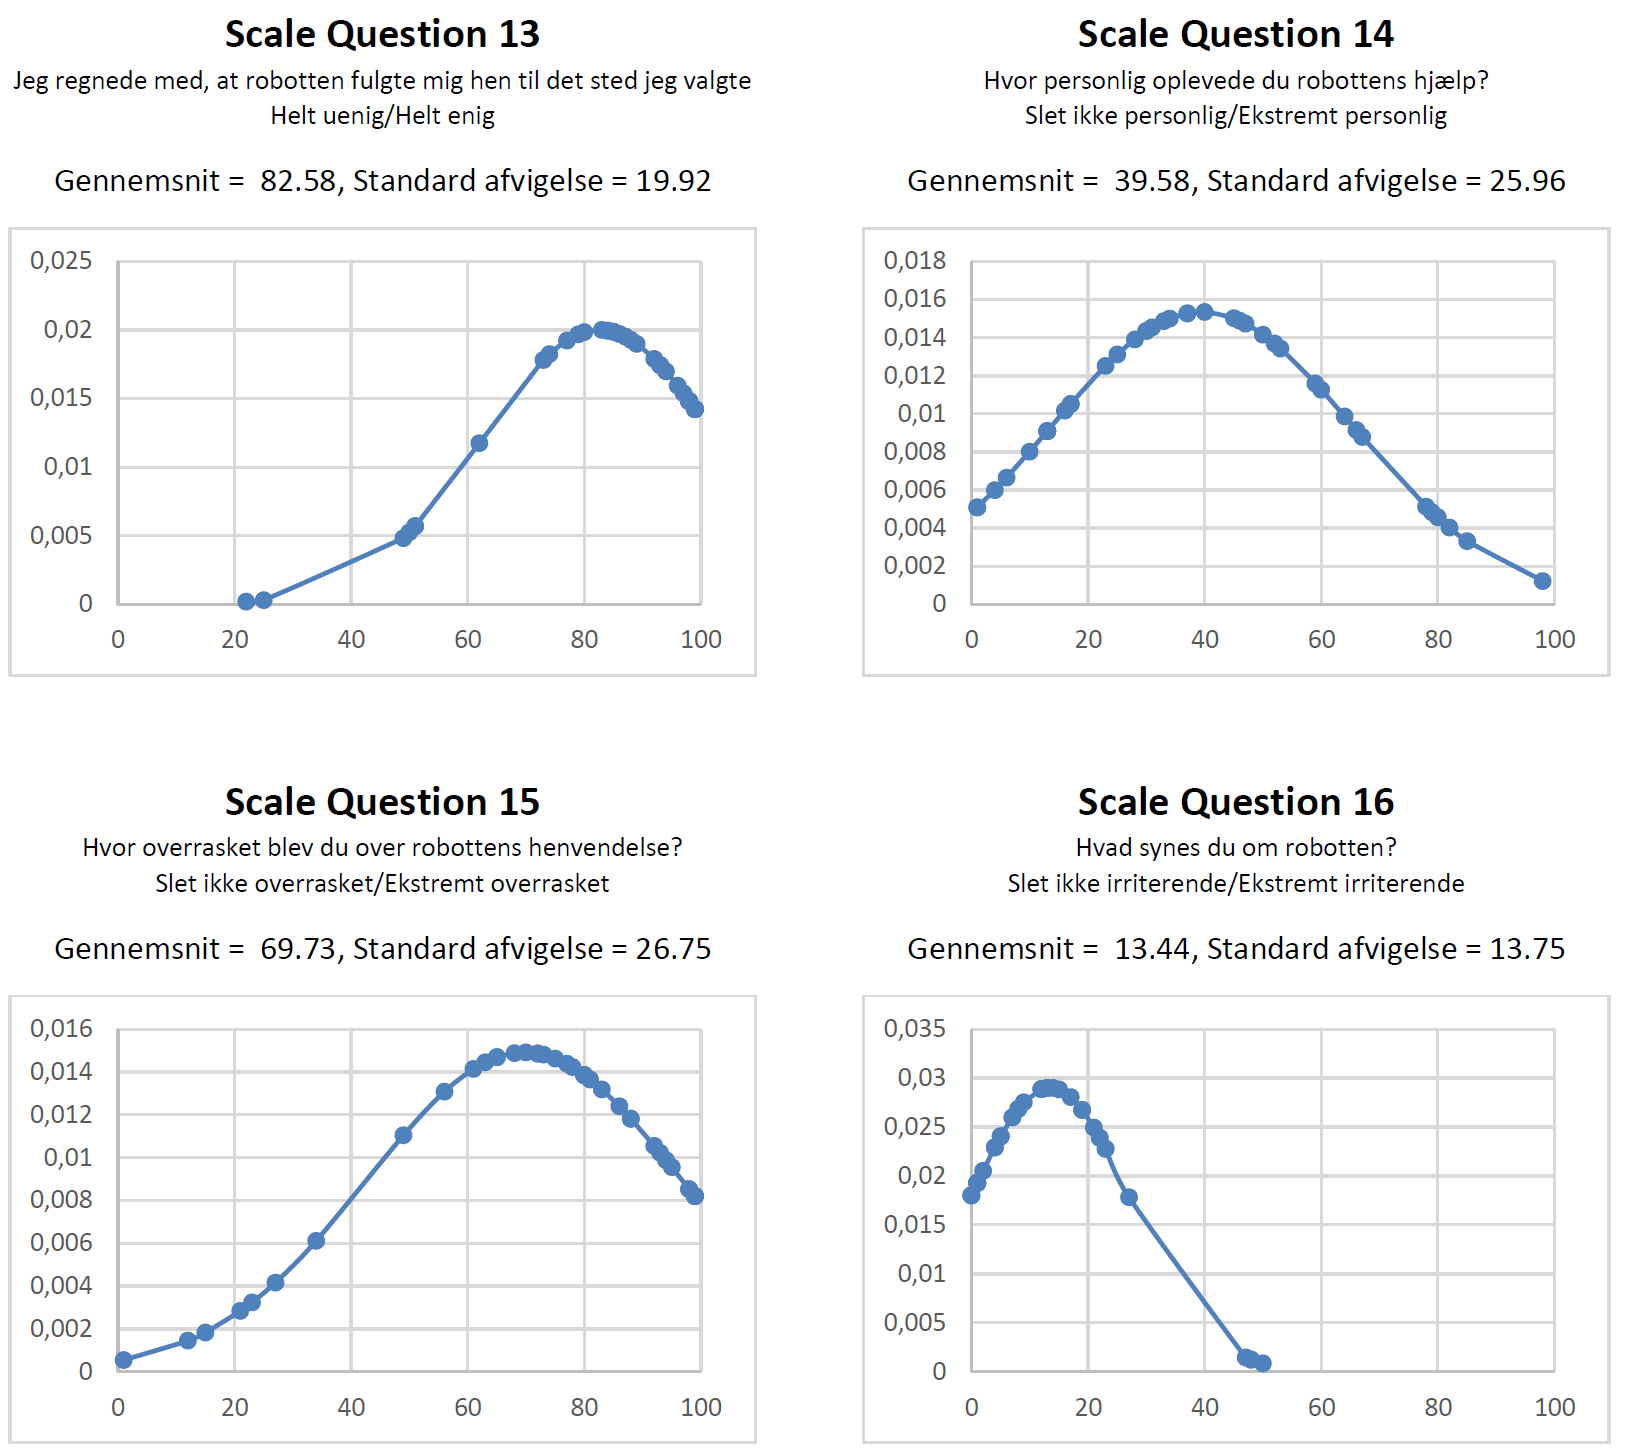
\includegraphics[width =\textwidth]{Figure/DatabehandlingSkalaer/FordelingSkala13_16} 
\caption{Fordelingen af besvarelserne til Scale Question 13-16}
\label{fig:FordelingSkala13_16}
\end{figure}
\noindent

Fordelingen på SQ13 virker også venstre skævvreden. Se \autoref{fig:FordelingSkala13_16}. Folk virker generelt til at stole på, at robotten leder dem det rette sted hen. Ligesom SQ1 virker SQ14 oprigtigt normalfordelt, da datapunkterne er jævnt fordelt. Dog er de begge to meget flade og ar en høj standadafvigelse ligesom resten af fordelingerne pånær SQ7. Generelt synes folk ikke, at robotten er irriterende selvom de blev overraskede over dens henvendelse. 

\begin{figure}[H]
\centering
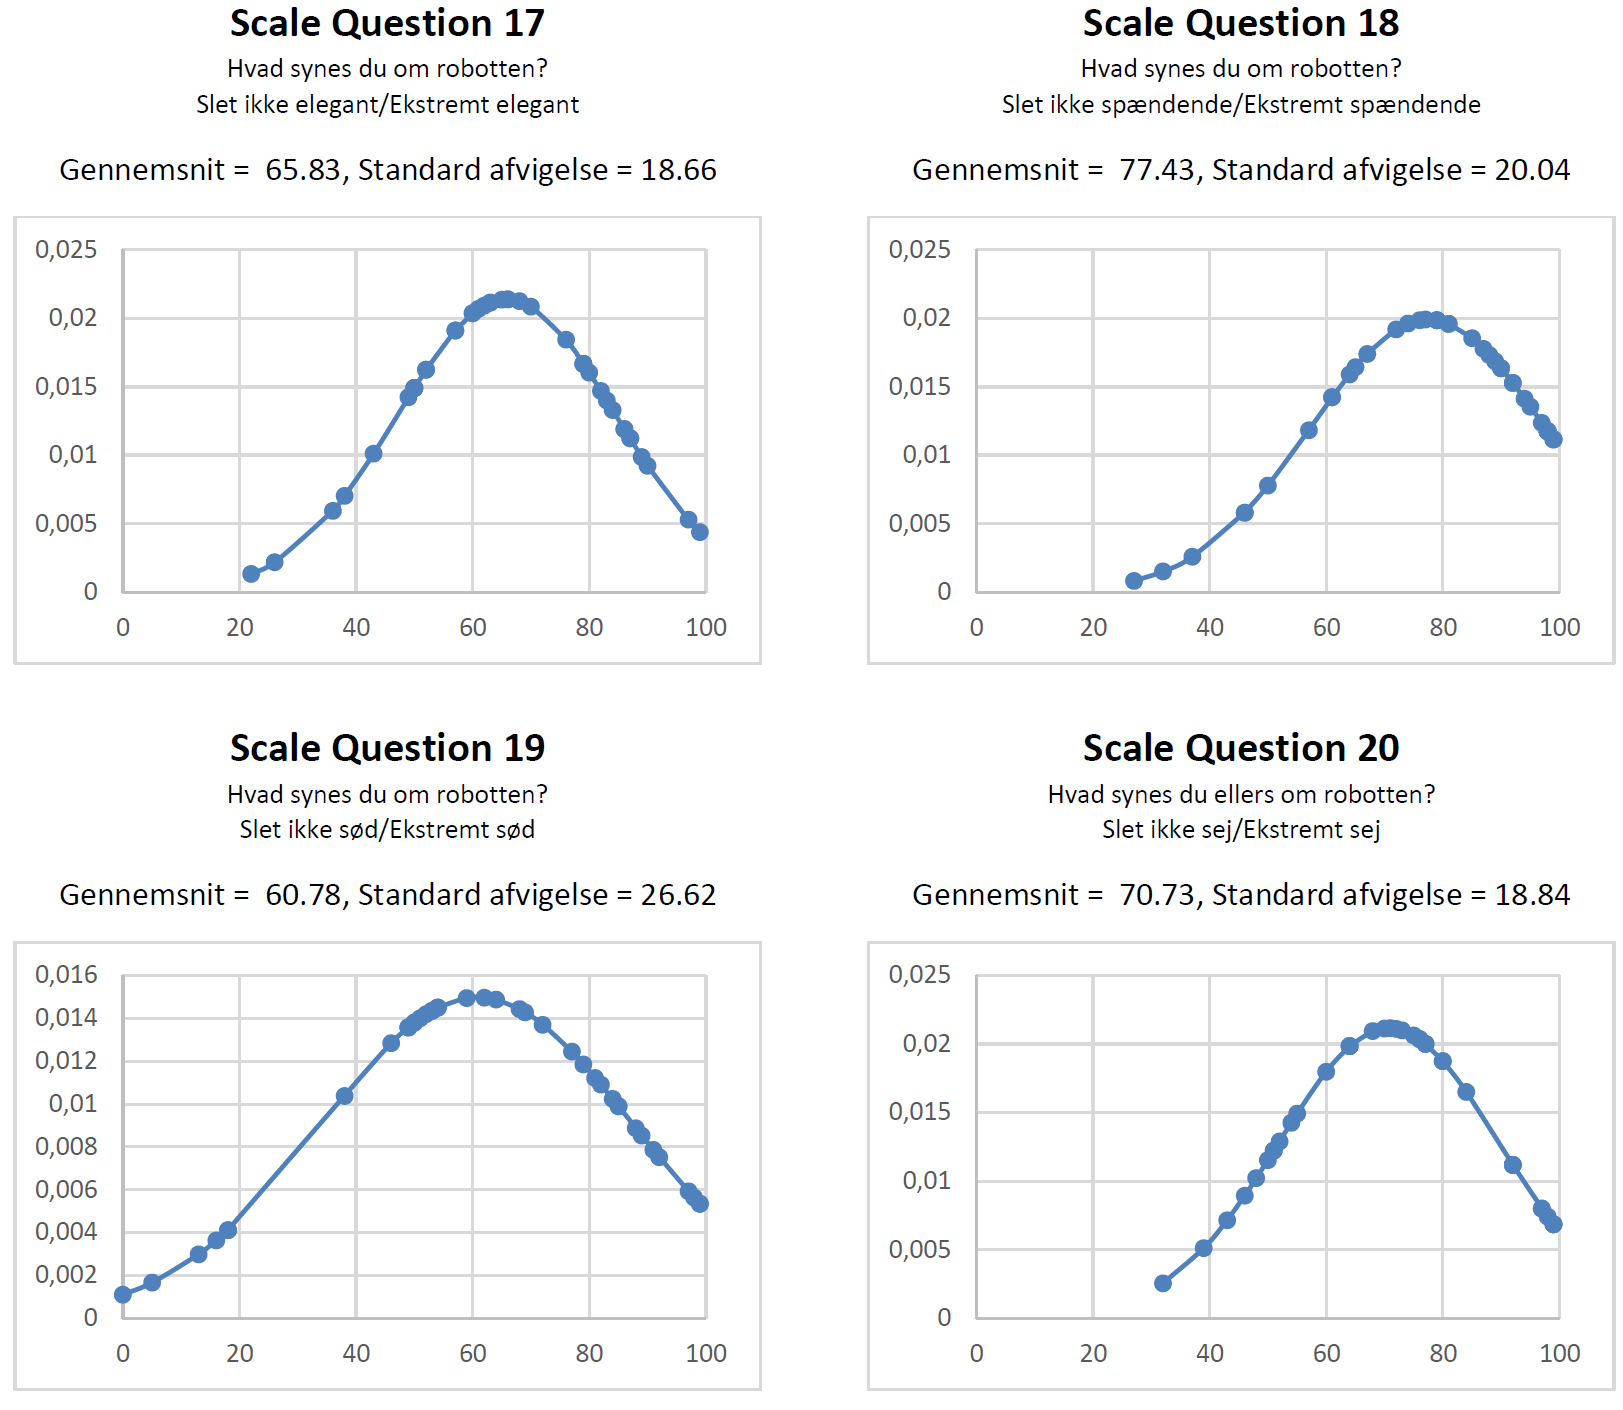
\includegraphics[width =\textwidth]{Figure/DatabehandlingSkalaer/FordelingSkala17_20} 
\caption{Fordelingen af besvarelserne til Scale Question 17-20}
\label{fig:FordelingSkala17_20}
\end{figure}
\noindent

Ved SQ17-20 ligger alle gennemsnit over midten på skalaen. Ser man på fordelingerne er robotten tenderende spændende, sej og elegant. SQ19 omhandlende Sød har en lidt større spredning hvilket måske kan skyldes, at ordet kan dække over flere forskellige ting. Dette blev også kommenteret af flere testpersoner under besvarelsen. 

\begin{figure}[H]
\centering
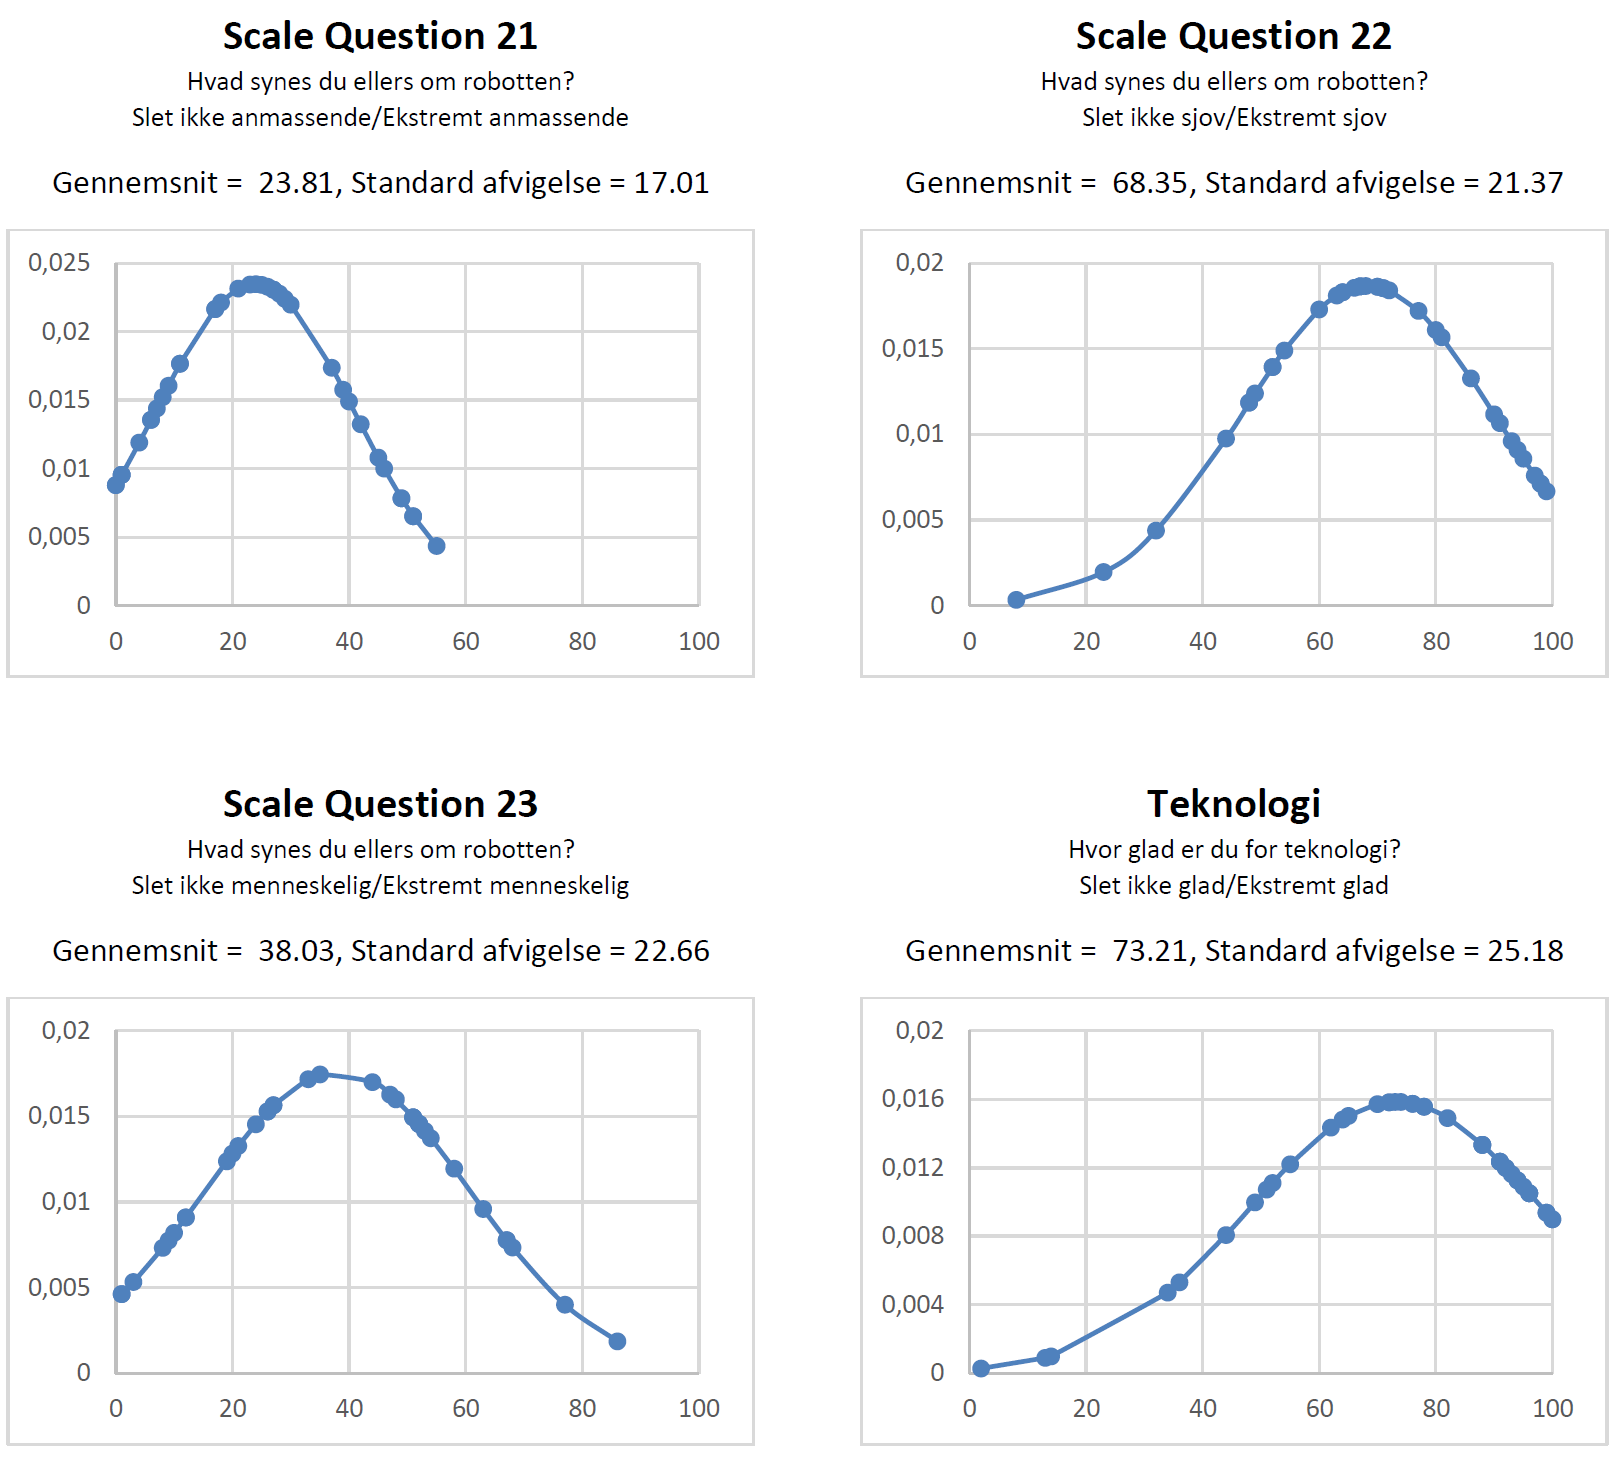
\includegraphics[width =\textwidth]{Figure/DatabehandlingSkalaer/FordelingSkala21_24} 
\caption{Fordelingen af besvarelserne til Scale Question 21-23 og teknologi}
\label{fig:FordelingSkala21_24}
\end{figure}
\noindent

På \autoref{fig:FordelingSkala21_24} ses, at data fordeler sig en del under midterpunktet på SQ21. Det betyder, at robotten for de fleste ikke har virket anmassende. SQ22 viser også en tendes, at folk synes robotten er sjov. Data er venstre skævvreden.  SQ23 viser en tendens, at folk ikke synes den virker menneskelig. Dog er der stadig del datapunkter over midterpunktet. Teknologi-fordelingen var en del af demografisiden præsenteret på et papir. Den viser, at størstedelen af besvarelserne kom fra folk, der vurderer, at de er glade for teknologi. Dette kan have en indflydelse på hvorfor der generelt har være positive besvarelser igennem datasættet. 

